\section{Join Queries}
\hrulefill

\begin{itemize}
    \item Get the team name and manager name for each team
\end{itemize}

\begin{lstlisting}[ caption={ Query 1},label={lst:q-1}]
    SELECT t.Team_Name, m.Manager_Name
    FROM Team t
    JOIN Manager m ON t.Manager_ID = m.Manager_ID;
\end{lstlisting}
\begin{figure}[H]
    \centering
    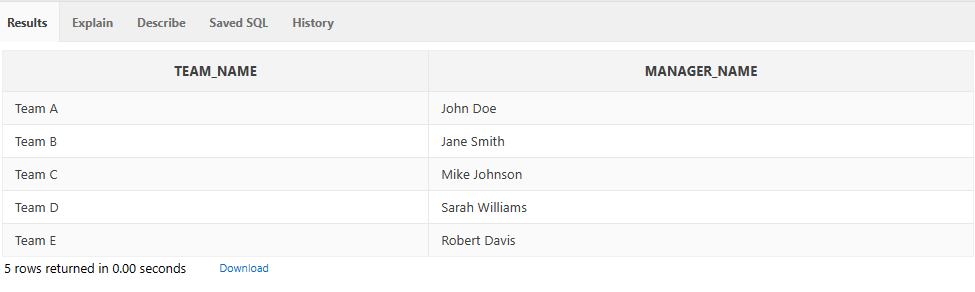
\includegraphics[width=0.9\textwidth]{images/dml/Joinq/q1.png}
    \caption{Result of Query 1}
\end{figure}
%%%
\begin{itemize}
    \item Retrieve the player name, team name, and country for each player
\end{itemize}
\begin{lstlisting}[ caption={ Query 2},label={lst:q-2}]
    SELECT p.Player_Name, t.Team_Name, t.Team_Country
    FROM Player p
    JOIN Player_Team pt ON p.Player_ID = pt.Player_ID
    JOIN Team t ON pt.Team_ID = t.Team_ID;
\end{lstlisting}
\begin{figure}[H]
    \centering
    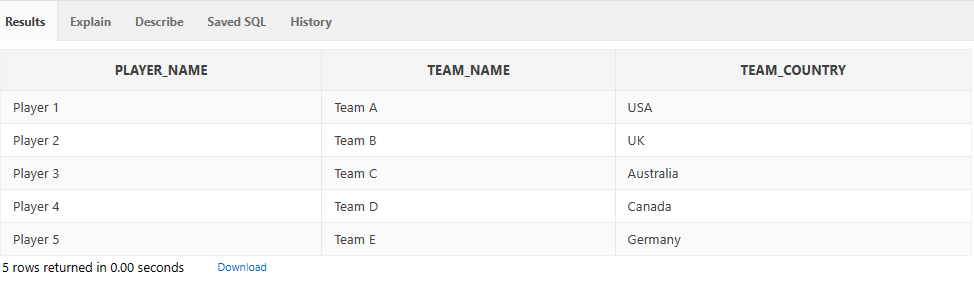
\includegraphics[width=0.9\textwidth]{images/dml/Joinq/q2.png}
    \caption{Result of Query 2}
\end{figure}
%%%
\clearpage
\begin{itemize}
    \item Get the content creator name, social media name, and email for each content creator
\end{itemize}
\begin{lstlisting}[ caption={ Query 3},label={lst:q-3}]
    SELECT cc.ContentCreator_Name, sm.SocialMedia_Name, sm.SocialMedia_Email
    FROM ContentCreator cc
    JOIN SocialMedia sm ON cc.SOCIALMEDIA_ID = sm.SocialMedia_ID;
\end{lstlisting}
\begin{figure}[H]
    \centering
    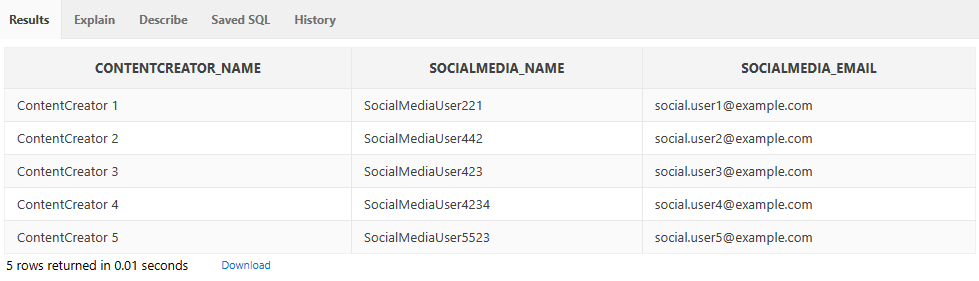
\includegraphics[width=1\textwidth]{images/dml/Joinq/q3.png}
    \caption{Result of Query 3}
\end{figure}
\clearpage